\documentclass[a4paper,14pt,russian]{extreport} \usepackage{extsizes}
\usepackage{cmap} 
\usepackage[T2A]{fontenc}
\usepackage[utf8]{inputenc}
\usepackage[russian]{babel}
\usepackage{pscyr}
\usepackage{graphicx}  \usepackage{amssymb,amsfonts,amsmath,amsthm}  \usepackage{indentfirst} \usepackage[usenames,dvipsnames]{color}
\usepackage{makecell}
\usepackage{multirow}
\usepackage{ulem} 
\linespread{1.3} 
\renewcommand{\rmdefault}{ftm}
\frenchspacing
\usepackage{fancyhdr}
\pagestyle{fancy}
\fancyhf{}
\fancyhead[R]{\thepage}
\fancyheadoffset{0mm}
\fancyfootoffset{0mm}
\setlength{\headheight}{17pt} \renewcommand{\headrulewidth}{0pt} \renewcommand{\footrulewidth}{0pt} \fancypagestyle{plain}{\fancyhf{} \rhead{\thepage}}
\setcounter{page}{2} % начать нумерацию страниц с №2
\usepackage[tableposition=top]{caption}
\usepackage{subcaption}
\DeclareCaptionLabelFormat{gostfigure}{Рисунок #2} \DeclareCaptionLabelFormat{gosttable}{Таблица #2} \DeclareCaptionLabelSeparator{gost}{~---~}
\captionsetup{labelsep=gost} 
\captionsetup[figure]{labelformat=gostfigure}
\captionsetup[table]{labelformat=gosttable} \renewcommand{\thesubfigure}{\asbuk{subfigure}}
\usepackage{titlesec} 
\titleformat{\chapter}[display]
{\filcenter}
{\MakeUppercase{\chaptertitlename} \thechapter}     {8pt}    
{\bfseries}{} 
\titleformat{\section}
{\normalsize\bfseries}
{\thesection}{1em}{}
\titleformat{\subsection}     
{\normalsize\bfseries}
{\thesubsection}     
{1em}{}
\titlespacing*{\chapter}{0pt}{-30pt}{8pt} \titlespacing*{\section}{\parindent}{*4}{*4} \titlespacing*{\subsection}{\parindent}{*4}{*4}
\usepackage{geometry}
\geometry{left=3cm}
\geometry{right=1.5cm}
\geometry{top=2.4cm}
\geometry{bottom=2.4cm}
\usepackage{enumitem}
\makeatletter  
\AddEnumerateCounter{\asbuk}{\@asbuk}{м)} 
\makeatother
\setlist{nolistsep}
\renewcommand{\labelitemi}{-} \renewcommand{\labelenumi}{\asbuk{enumi})} \renewcommand{\labelenumii}{\arabic{enumii})}
\newcommand{\empline}{\mbox{} \newline}
\newcommand{\likechapterheading}[1]{
\begin{center}
	   \textbf{\MakeUppercase{#1}}
\end{center}
\empline}
\sloppy
\newcommand{\jj}{\righthyphenmin=20 \justifying}
\usepackage{tocloft}
\renewcommand{\cfttoctitlefont}{\hspace{0.38\textwidth} \bfseries\MakeUppercase}
\renewcommand{\cftbeforetoctitleskip}{-1em}
\renewcommand{\cftaftertoctitle}{\mbox{}\hfill \\ 
\mbox{}\hfill{\footnotesize Стр.}\vspace{-2.5em}} \renewcommand{\cftchapfont}{\normalsize\bfseries \MakeUppercase{\chaptername} } \renewcommand{\cftsecfont}{\hspace{31pt}} \renewcommand{\cftsubsecfont}{\hspace{11pt}} \renewcommand{\cftbeforechapskip}{1em} 
\renewcommand{\cftparskip}{-1mm} \renewcommand{\cftdotsep}{1} \setcounter{tocdepth}{2} % задать глубину оглавления — до subsection включительно
\makeatletter
\renewcommand{\@dotsep}{2}     \newcommand{\l@likechapter}[2]{{\bfseries\@dottedtocline{0}{0pt}{0pt}{#1}{#2}}} \makeatother\newcommand{\likechapter}[1]{       
 \likechapterheading{#1}    
	 \addcontentsline{toc}{likechapter}{\MakeUppercase{#1}}}
\begin{document}
	\chapter{Разработка ПО}
	\section{Формирование алгоритма управления}
	Сетевая архитектура представлена на Рисунке 1.
	\begin{figure}[h]
		\centering		 
		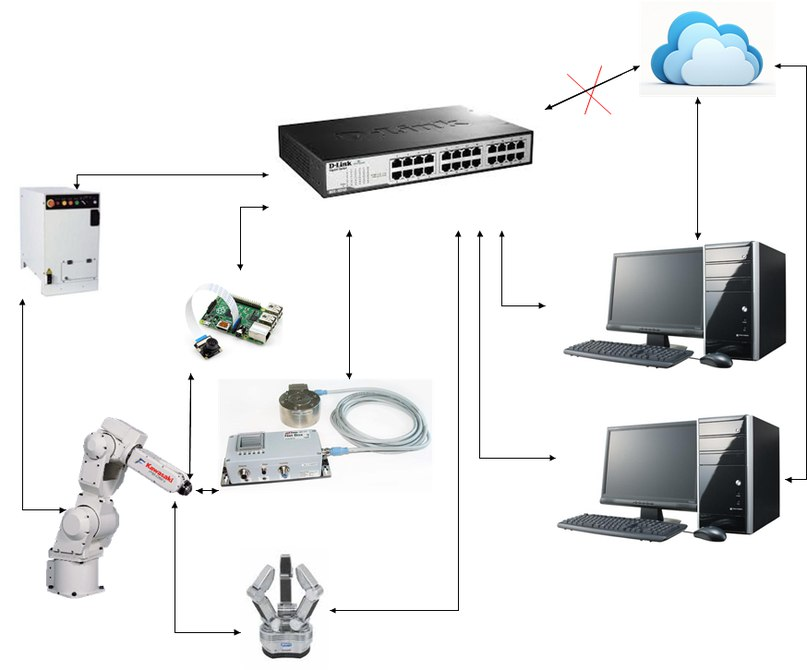
\includegraphics[width=5.5in]{./img/img42.jpg}	
		\caption{Сетевая архитектура}
		\label{fig_img51}
	\end{figure}
	
	У робота есть всего две группы параметров позиционирования: 
	1) углы поворотов шести джоинтов 
	2) Положение фланца, заданное в x,y,z координатах, и его ориентация, заданная в o,a,t углах  Эйлера в zyz конвенции.
	
	Т.к. робот получает управляющие команды по протоколу tcp ip, и контроль безошибочности передачи заложен в самом протоколе, то нам остаётся разработать собственный формат посылки.
	\section{Структура посылки}
	 Т.к. при позиционировании робот использует 6 величин, то будем строить посылку следующим образом.
	 
	 В силу функциональных особенностей внутреннего языка программирования контроллеров RoboticAS, самым оптимальным способом передачи данных по протоколу TCP IP является отправка символьных строк, содержащих в себе данные, разделённых пробелом (разделительным символом).  Единственное требование к такому представлению - это чтобы каждое число было представлено шестью символами. В случае, если число меньше 105, то недостающие разряды должны быть заполнены цифрой 0. Например, число 123 должно быть представлено в выходной строке, как 000123.
	 Минимальная единица посылки, называемая кадром, - это целое число. 
	 
	  Т.к. при использовании протокола tcp ip все символы строки гарантированно будут доставлены от передатчика к приёмнику, то механизм обработки входящих сообщений можно строить следующим образом: все входящие символы добавляются в буфер с конца, как только длина буфера превышает число n=k*w, где k - кол-во кадров в посылке, w - размер кадра в символах, то из буфера берутся первые n символов и переводятся в k целых чисел.
	  
	 Т.к. параметров позиционирования у робота-манипулятора шесть, то в состав посылки заложим 9 кадров.
	 
	 	\begin{figure}[ht]
	 		\centering		 
	 		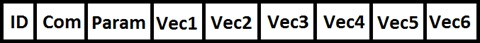
\includegraphics{./img/img41.jpg}	
	 		\caption{
	 			\textbf{ Структура посылки:} 				
	 				ID- уникальный  номер управляющей команды(id);	 				
	 				Com - номер управляющей команды;	 				
	 				Param- параметр управляющей команды(запасной);	 				
	 				Vec1...Vec6 - вектор параметров управляющей команды}     
	 		\label{fig_img51}
	 	\end{figure}
	 		
	 \section{Управление Кавасаки}
	 Всего есть три основных группы управления:
	 \begin{enumerate}  

		 \item{По положению. Вектор параметров имеет следующую структуру: 
	\begin{itemize}
	 \item{Vec1 – X координата фланца}
	 \item{Vec2 – Y координата фланца}
	 \item{ Vec3 – Z координата фланца}
	 \item{Vec4 – O угол Эйлера}
	 \item{Vec5 – A угол Эйлера} 
  	\item{ Vec6 – T угол Эйлера}
	\end{itemize}
	 }
	 \item{По абсолютным углам поворота джоинтов: i-ая координата отвечает за поворот  i-го джоинта.}
	 \item{По относительным углам поворота джоинтов:  i-ая координата отвечает  за поворот  i-го джоинта.}
	\end{enumerate}
	 
	 Внутренняя программа контролера построена следующим образом: запущено 3 параллельных процесса: первый в бесконечном цикле отправляет данные о положении фланца, его ориентации и углах поворота шести джоинтов. Второй процесс в в бесконечном цикле проверяет, не пришло ли новых символов и по каналу связи и добавляет их к буфферу. Третий  процесс в бесконечном цикле обрабатывает входящие управляющие команды и запускает вспомогательные программы внутреннего управления, если такое управление было вызвано.
 	 
	 \section{Внешние управляющие программы.}
	 \begin{enumerate}  
	  \item{	Вывод робота в заданную точку по координатам (X,Y,Z,O,A,T). В вектор параметров передаются соответствующие координаты. }
	  \item{	Вывод робота в заданную конфигурацию поворотов джоинтов. В вектор параметров передаются соответствующие углы поворота джоинтов.}
	  \item{	Вывод робота в заданную конфигурацию относительных поворотов джоинтов. В вектор параметров передаются соответствующие углы поворотов джоинтов.
	 При получении любой из первых трёх команд робот сразу же запускает внутреннюю команду перемещения. Поле Param остаётся нулевым.}
	  \item{	Передача значений показаний силомоментного датчика в базовой системе координат (преобразование реальных показаний датчиков производится на стороне PC). Поле Param остаётся нулевым.}
	  \item{	Задание скоростей и ускорений. Поле Param остаётся нулевым, значения vec1-vec4 следующие: ускорение в процентах, замедление в процентах, модульная скорость в процентах, механическая скорость в мм/с. Реальная скорость робота является произведением механической на модульную скорости.}
	  \item{	Задание коэффициентов регулирования. При поле Param, равном нулю задаются пропорциональные коэффициенты kx,ky,kz,kmx,kmy,kmz, при поле Param, равном 1 задаются интегральные коэффициенты  ix,iy,iz,imx,imy,Imz.}
	  \item{	Запуск программы force feedback. При Param, равном 0 – запускает режим стабилизации показаний x,y,z компонент силомоментного датчика в нулевых значениях  за счёт смещений по x,y,z осям. ForceFeedBackPosition. При Param равном 1 – запускается режим стабилизации mx,my,mz показаний силомоментного датчика в нулевых значениях. ForceFeedBackOrientation. При Param равном 2 останавливается выполнение force feedback.}
	\end{enumerate}   
	
	\section{Работа Force Feedback}
	
	Из-за низкой производительности контроллера Kawasaki все математические вычисления производятся на ПК. Контроллер получает уже преобразованные значения x,y,z компонент силы в базисе базовой системы координат. Mx, My и Mz – моменты, возникающие вдоль осей x,y и z базовой системы координат. Force feedback Position реализует при помощи ПИ регулятора, где за ошибку берётся значение x,y,z компонент силомоментного датчика. Выходом регулятора  является  новое положение робота на следующей итерации главного цикла программы.  
	
	Force FeedBack Orientation планируется организовать более сложным способом. Также строится ПИ регулятор, за ошибку берутся показания моментов Mx, My, Mz, На выходе мы получаем углы поворота относительно осей x,y,z базовой системы координат.
	
	Итого, мы имеем 3 задачи:
	\begin{enumerate}   
	\item{	Преобразование значения силы  из системы координат датчика в базовую систему координат и компенсация силы тяжести инструмента. }
	\item{	Преобразование значений моментов из системы координат датчика в базовую систему координат и компенсация момента силы тяжести инструмента.}
	\item{	Поворот инструмента вдоль ортов базовой системы координат.}
	\end{enumerate}   
	
\end{document}